\section{Cơ chế Chú ý trong CNN: SE-Net, CBAM và Non-local Networks}
\label{sec:attention_in_cnn}

\subsection{Giới thiệu: Không phải mọi Đặc trưng đều bình đẳng}
\label{subsec:attention_intro}

Sau khi đã nắm vững các kiến trúc CNN hiện đại như ResNet và EfficientNet, chúng ta có thể nhận ra một hạn chế tinh tế nhưng quan trọng. Trong một lớp tích chập thông thường, tất cả các kênh đặc trưng (feature channels) và mọi vị trí không gian đều được xử lý như nhau—không có sự ưu tiên, không có sự \textit{tập trung}. Mạng "nhìn" đều tất cả mọi nơi trên ảnh với cùng một mức độ quan tâm.

Nhưng não bộ con người không hoạt động như vậy.

Khi bạn tìm kiếm chìa khóa trong căn phòng lộn xộn, ánh mắt bạn không quét đều từng centimet vuông. Thay vào đó, nó \textit{tập trung} vào những nơi có khả năng nhất—trên bàn, gần cửa, cạnh ghế. Khi bạn nhận ra giọng nói của bạn bè trong một bữa tiệc ồn ào, não bộ bạn \textit{lọc bỏ} hầu hết âm thanh xung quanh và \textit{chú ý} vào tần số giọng nói đặc trưng.

\textbf{Cơ chế Chú ý (Attention Mechanism)} trong mạng nơ-ron tích chập là nỗ lực hiện thực hóa nguyên lý sinh học này vào thế giới tính toán. Ý tưởng cốt lõi: \textit{học cách cân bằng lại} (recalibrate) tầm quan trọng của các kênh đặc trưng hoặc các vị trí không gian khác nhau, để mạng có thể tập trung vào những phần thực sự có ý nghĩa.

\begin{mdframed}[style=infobox]
    \textbf{Vị trí trong lịch sử}

    Các cơ chế chú ý trong CNN (2018--2020) chính là \textit{cầu nối tư duy} giữa kỷ nguyên CNN thuần túy và kỷ nguyên Transformer. Chúng chứng minh rằng tư duy "chú ý có chọn lọc" là mạnh mẽ ngay cả trong kiến trúc tích chập, và dọn đường cho sự ra đời của Vision Transformer (sẽ học ở Chương 4).
\end{mdframed}

\subsection{Squeeze-and-Excitation Networks (SE-Net): Chú ý theo Kênh}
\label{subsec:senet}

\subsubsection{Động lực: Các kênh đặc trưng không đều nhau}
\label{subsubsec:senet_motivation}

Xét một lớp tích chập tạo ra $C$ kênh đặc trưng. Một số kênh có thể đang mã hóa thông tin rất liên quan đến tác vụ hiện tại (ví dụ: màu da khi nhận dạng khuôn mặt), trong khi các kênh khác có thể mã hóa các đặc trưng ít quan trọng hơn (ví dụ: kết cấu nền). Nếu mạng có thể \textit{học cách nâng cao} những kênh quan trọng và \textit{ức chế} những kênh kém quan trọng hơn, tổng thể hiệu năng sẽ tăng lên.

Đây chính là ý tưởng của Squeeze-and-Excitation Networks (SENet) \cite{Hu2018}, giành chiến thắng tại cuộc thi ImageNet 2017.

\subsubsection{Kiến trúc SE Block}
\label{subsubsec:senet_architecture}

Một SE block có thể được cắm vào (plug-in) bất kỳ kiến trúc CNN nào và hoạt động theo ba bước:

\begin{enumerate}
    \item \textbf{Squeeze — Nén thông tin không gian:}
    Cho bản đồ đặc trưng đầu vào $\mathbf{X} \in \mathbb{R}^{H \times W \times C}$, bước Squeeze sử dụng \textbf{Global Average Pooling} để "nén" mỗi kênh thành một con số đại diện duy nhất:
    \[
        z_c = \frac{1}{H \times W} \sum_{i=1}^{H} \sum_{j=1}^{W} X_c(i, j)
    \]
    Kết quả là một vector $\mathbf{z} \in \mathbb{R}^C$, trong đó $z_c$ mã hóa \textit{mức độ hoạt động trung bình} của kênh thứ $c$. Đây là "thống kê toàn cục" của từng kênh.

    \item \textbf{Excitation — Học tầm quan trọng của từng kênh:}
    Vector $\mathbf{z}$ được đưa qua một mạng nhỏ gồm hai lớp fully-connected để học tương quan giữa các kênh và tạo ra một tập hợp trọng số $\mathbf{s}$:
    \[
        \mathbf{s} = \sigma\!\left(W_2 \cdot \delta\!\left(W_1 \mathbf{z}\right)\right)
    \]
    trong đó $\delta$ là ReLU, $\sigma$ là Sigmoid (đảm bảo trọng số trong $(0, 1)$), và $W_1, W_2$ là các ma trận trọng số với chiều giảm dần theo tỉ lệ $r$ (reduction ratio, thường $r=16$) để tiết kiệm tham số.

    \item \textbf{Scale — Áp dụng trọng số lên bản đồ đặc trưng:}
    Mỗi kênh của $\mathbf{X}$ được nhân với trọng số tương ứng trong $\mathbf{s}$:
    \[
        \tilde{X}_c = s_c \cdot X_c
    \]
\end{enumerate}

\begin{center}
    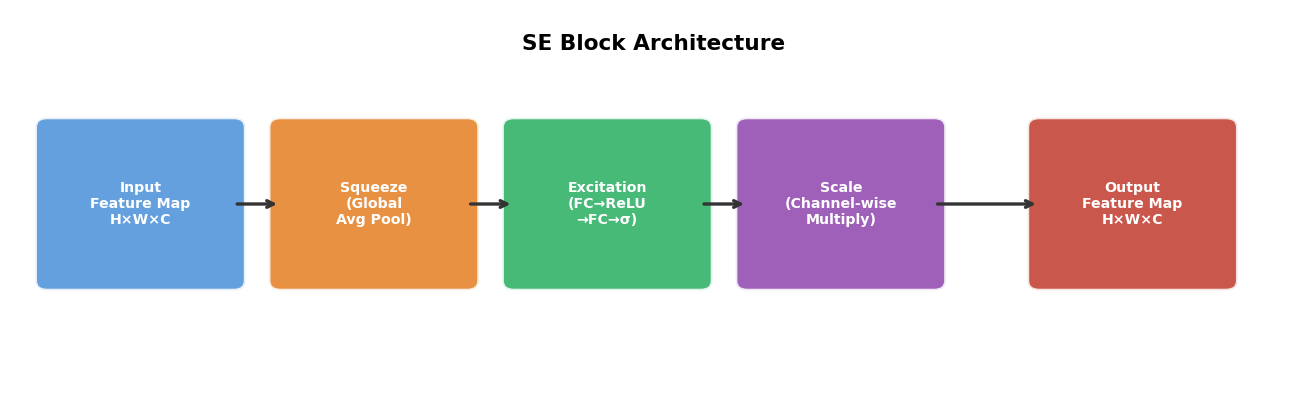
\includegraphics[width=0.9\textwidth]{images/senet_block.png}
    \captionof{figure}{Kiến trúc SE Block. Bước Squeeze nén thông tin không gian của từng kênh bằng Global Average Pooling. Bước Excitation học tầm quan trọng của từng kênh qua hai lớp FC. Bước Scale nhân lại các trọng số đó lên bản đồ đặc trưng gốc.}
    \label{fig:senet_block}
\end{center}

\begin{mdframed}[style=infobox]
    \textbf{Trực giác: SE Block như một "bộ điều chỉnh âm lượng"}

    Hãy hình dung 512 kênh đặc trưng như 512 nhạc cụ trong một dàn nhạc. Bước Squeeze "nghe" toàn bộ bản nhạc và tóm tắt "âm lượng" của từng nhạc cụ. Bước Excitation học cách điều chỉnh: nhạc cụ nào nên được "vặn to hơn" và nhạc cụ nào nên "bị hạ xuống" để tạo ra bản nhạc hay nhất cho bài tác vụ hiện tại. Bước Scale thực sự thực hiện việc điều chỉnh đó.
\end{mdframed}

SE block cực kỳ nhẹ (chỉ thêm $\frac{2C^2}{r}$ tham số), nhưng mang lại cải thiện đáng kể: SE-ResNet-50 vượt trội ResNet-50 trên ImageNet với chi phí tính toán tăng thêm không đáng kể.

\subsection{CBAM: Chú ý theo cả Kênh lẫn Không gian}
\label{subsec:cbam}

\subsubsection{Mở rộng tư duy: Chú ý Không gian}
\label{subsubsec:cbam_motivation}

SE-Net chỉ tập trung vào câu hỏi \textit{"Kênh nào quan trọng?"}. Nhưng có một câu hỏi bổ sung cũng quan trọng không kém: \textit{"Vùng nào trong ảnh quan trọng?"}

CBAM (Convolutional Block Attention Module) \cite{Woo2018} mở rộng SE-Net bằng cách kết hợp \textbf{cả hai dạng chú ý}: chú ý theo kênh (channel attention) và chú ý theo không gian (spatial attention), áp dụng tuần tự.

\subsubsection{Kiến trúc CBAM}
\label{subsubsec:cbam_architecture}

\textbf{Bước 1 — Channel Attention Module (giống cải tiến SE):}
Tương tự SE-Net, nhưng CBAM sử dụng cả Max Pooling lẫn Average Pooling để thu thập thống kê kênh toàn cục, rồi kết hợp chúng qua một mạng chia sẻ trọng số (shared MLP):
\[
    \mathbf{M}_c = \sigma\!\left(\text{MLP}(\text{AvgPool}(\mathbf{X})) + \text{MLP}(\text{MaxPool}(\mathbf{X}))\right)
\]

\textbf{Bước 2 — Spatial Attention Module:}
Sau khi áp dụng channel attention, bản đồ đặc trưng $\mathbf{X}' = \mathbf{M}_c \otimes \mathbf{X}$ tiếp tục được đưa qua spatial attention module. Mô-đun này nén theo chiều kênh (trả về thông tin không gian) và học \textit{vị trí nào trong ảnh} cần chú ý:
\[
    \mathbf{M}_s = \sigma\!\left(f^{7\times7}\!\left([\text{AvgPool}_C(\mathbf{X}');\, \text{MaxPool}_C(\mathbf{X}')]\right)\right)
\]
trong đó $[\,;\,]$ là ghép nối (concatenation), $f^{7 \times 7}$ là tích chập $7 \times 7$, và $\text{AvgPool}_C, \text{MaxPool}_C$ là pooling dọc theo chiều kênh.

Đầu ra cuối cùng: $\tilde{\mathbf{X}} = \mathbf{M}_s \otimes \mathbf{X}'$.

\begin{center}
    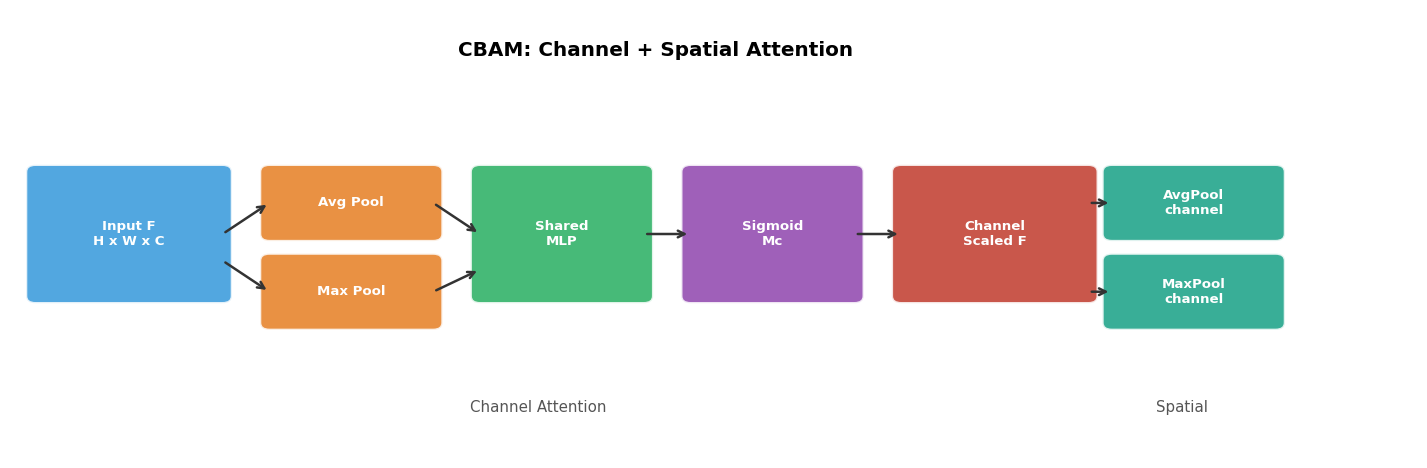
\includegraphics[width=1.0\textwidth]{images/cbam_diagram.png}
    \captionof{figure}{Kiến trúc CBAM. Hai module chú ý được áp dụng tuần tự: Channel Attention Module (trái) học tầm quan trọng của từng kênh, và Spatial Attention Module (phải) học tầm quan trọng của từng vị trí không gian.}
    \label{fig:cbam_diagram}
\end{center}

\subsection{Non-local Networks: Tương tác Tầm xa}
\label{subsec:nonlocal_networks}

\subsubsection{Hạn chế của Tích chập: Bị nhốt trong Vùng lân cận}
\label{subsubsec:nonlocal_motivation}

Cả SE-Net và CBAM đều vẫn dựa trên tích chập—một phép toán \textit{cục bộ}. Một lớp tích chập $3 \times 3$ chỉ kết nối một pixel với $3 \times 3 = 9$ pixel lân cận. Để kết nối một pixel với một pixel ở cách xa, mạng cần nhiều lớp tích chập xếp chồng.

Điều này tạo ra một vấn đề đặc biệt trong video: để nhận ra rằng hành động "bắt tay" liên quan đến sự di chuyển của hai cánh tay ở hai vị trí khác nhau trong khung hình, mạng cần nắm bắt sự phụ thuộc tầm xa (long-range dependency) một cách hiệu quả.

\textbf{Non-local Networks} \cite{Wang2018nonlocal} giải quyết điều này bằng cách tính toán phản hồi tại một vị trí như là \textit{tổng có trọng số của tất cả các vị trí khác} trong cùng bản đồ đặc trưng—đây chính là bản chất của \textbf{self-attention}.

\subsubsection{Phép toán Non-local}
\label{subsubsec:nonlocal_operation}

\begin{equation}
    \mathbf{y}_i = \frac{1}{\mathcal{C}(\mathbf{x})} \sum_{\forall j} f(\mathbf{x}_i, \mathbf{x}_j) \cdot g(\mathbf{x}_j)
    \label{eq:nonlocal_mean}
\end{equation}

trong đó:
\begin{itemize}
    \item $\mathbf{x}_i$ là đặc trưng tại vị trí $i$ (có thể là pixel, hay điểm trong không-thời gian cho video).
    \item $f(\mathbf{x}_i, \mathbf{x}_j)$ là hàm đo lường độ tương đồng giữa vị trí $i$ và $j$ (thường là dot product hay Gaussian).
    \item $g(\mathbf{x}_j)$ là biểu diễn của vị trí $j$ (thường là phép chiếu tuyến tính).
    \item $\mathcal{C}(\mathbf{x})$ là hệ số chuẩn hóa.
\end{itemize}

Phép toán này \textit{kết nối mọi vị trí với mọi vị trí khác} trong một bước duy nhất—không cần xếp chồng nhiều lớp tích chập.

\begin{mdframed}[style=infobox]
    \textbf{Kết nối đến Transformer}

    Phép toán Non-local Mean chính là \textbf{Self-Attention}—trái tim của kiến trúc Transformer. Khi bạn học về Vision Transformer ở Chương 4, bạn sẽ nhận ra rằng attention là sự tổng quát hóa của ý tưởng non-local này, được đưa lên một tầm cao và tỉ lệ (scale) hoàn toàn mới.
\end{mdframed}

\subsection{Tóm tắt: Con đường từ CNN đến Transformer}
\label{subsec:attention_cnn_summary}

Ba cơ chế chú ý trên đại diện cho một sự tiến hóa liên tục của tư duy:

\begin{enumerate}
    \item \textbf{SE-Net (2018):} "Kênh nào quan trọng?" — Chú ý 1D theo chiều kênh.
    \item \textbf{CBAM (2018):} "Kênh nào \textit{và} vùng nào quan trọng?" — Chú ý 1D + 2D.
    \item \textbf{Non-local Networks (2018):} "Vị trí nào có liên quan đến vị trí nào?" — Chú ý tầm xa toàn cục.
\end{enumerate}

Từ Non-local Networks đến Self-Attention của Transformer chỉ còn một bước nhỏ về mặt toán học, nhưng là một bước nhảy vọt về kiến trúc và khả năng mở rộng. Khi Dosovitskiy và cộng sự nhận ra rằng có thể \textit{thay thế toàn bộ CNN} bằng một chuỗi các phép self-attention, Vision Transformer (ViT) ra đời—và lịch sử CV sang trang mới.

\section*{Tài liệu tham khảo}
\begin{itemize}
    \item[1] Hu, J.; Shen, L.; Sun, G. Squeeze-and-Excitation Networks. In \textit{CVPR}, 2018.
    \item[2] Woo, S.; Park, J.; Lee, J.Y.; Kweon, I.S. CBAM: Convolutional Block Attention Module. In \textit{ECCV}, 2018.
    \item[3] Wang, X.; Girshick, R.; Gupta, A.; He, K. Non-local Neural Networks. In \textit{CVPR}, 2018.
\end{itemize}
